\documentclass[15pt,a5paper,reqno]{article}
\usepackage{hyperref}
\usepackage[warn]{mathtext}
\usepackage[utf8]{inputenc}
\usepackage[T2A]{fontenc}
\usepackage[russian]{babel}
\usepackage{amssymb, amsmath, multicol}
\usepackage{graphicx}
\usepackage[shortcuts,cyremdash]{extdash}
\usepackage{wrapfig}
\usepackage{gensymb}
\usepackage{floatflt}
\usepackage{lipsum}
\usepackage{verbatim}
\usepackage{concmath}
\usepackage{euler}
\usepackage{xcolor}
\usepackage{etoolbox}
\usepackage{fancyhdr}
\usepackage{subfiles}
\usepackage{enumitem}
\usepackage{amsthm}
\usepackage{indentfirst}
\usepackage{import}

\DeclareMathOperator{\sign}{sign}

\RequirePackage[ left     = 1.5cm,
  right    = 1.5cm,
  top      = 2.0cm,
  bottom   = 1.25cm,
  includefoot,
  footskip = 1.25cm ]{geometry}
\setlength    {\parskip}        { .5em plus .15em minus .08em }
%\setlength    {\parindent}      { .0em }
\renewcommand {\baselinestretch}{ 1.07 }

\fancyhf{}

\renewcommand{\footrulewidth}{ .0em }
\fancyfoot[C]{\texttt{\textemdash~\thepage~\textemdash}}

\makeatletter
\patchcmd\l@section{%
  \nobreak\hfil\nobreak
}{%
  \nobreak
  \leaders\hbox{%
    $\m@th \mkern \@dotsep mu\hbox{.}\mkern \@dotsep mu$%
  }%
  \hfill
  \nobreak
}{}{\errmessage{\noexpand\l@section could not be patched}}
\makeatother
\parindent = 1cm % отступ при красной строке⏎
\pagestyle{fancy}    
\renewcommand\qedsymbol{$\blacksquare$}

\newcommand{\when}[2]{
  \left. #1 \right|_{#2} \hspace
}
\renewcommand{\kappa}{\varkappa}
\RequirePackage{caption2}
\renewcommand\captionlabeldelim{}
\newcommand*{\hm}[1]{#1\nobreak\discretionary{}

\DeclareSymbolFont{T2Aletters}{T2A}{cmr}{m}{it}
{\hbox{$\mathsurround=0pt #1$}}{}}
% Цвета для гиперссылок
\definecolor{linkcolor}{HTML}{000000} % цвет ссылок
\definecolor{urlcolor}{HTML}{799B03} % цвет гиперссылок
 
\hypersetup{pdfstartview=FitH,  linkcolor=linkcolor,urlcolor=urlcolor, colorlinks=true}


%\setcounter{secnum[utf8x]depth}{0}

\begin{document}

% НАЧАЛО ТИТУЛЬНОГО ЛИСТА
\begin{center}
  {\small ФЕДЕРАЛЬНОЕ ГОСУДАРСТВЕННОЕ АВТОНОМНОЕ ОБРАЗОВАТЕЛЬНОЕ\\ УЧРЕЖДЕНИЕ ВЫСШЕГО ОБРАЗОВАНИЯ\\ МОСКОВСКИЙ ФИЗИКО-ТЕХНИЧЕСКИЙ ИНСТИТУТ\\ (НАЦИОНАЛЬНЫЙ ИССЛЕДОВАТЕЛЬСКИЙ УНИВЕРСИТЕТ)\\ ФИЗТЕХ-ШКОЛА РАДИОТЕХНИКИ И КОМПЬЮТЕРНЫХ ТЕХНОЛОГИЙ}\\
  \hfill \break
  \hfill \break
  \hfill \break
  \Huge{Работа 2.2.3. \\ Определение теплопроводности газов при атмосферном давлении}\\
\end{center}

\hfill \break
\hfill \break
\hfill \break
\hfill \break
\hfill \break
\hfill \break

\begin{flushright}
  \normalsize{Работу выполнил:}\\
  \normalsize{\textbf{Долгов Александр Алексеевич, группа Б01-106}}\\
\end{flushright}

\begin{center}
  \normalsize{\textbf{Долгопрудный, 2022}}
\end{center}


\thispagestyle{empty} % выключаем отображение номера для этой страницы

% КОНЕЦ ТИТУЛЬНОГО ЛИСТА

\newpage
\thispagestyle{plain}
\tableofcontents
\thispagestyle{plain}
\newpage

\section{Аннотация}

    В данной работе определяется коэффициент теплопроводности воздуха при постоянном атмосферном давлении и разных температурах. Для этого исследуется процесс теплоотдачи нити, нагреваемой током.
	
\section{Теоретические сведения}

    \subsection{Получение расчётной формулы}

    Теплопроводность - процесс выравнивания температуры в теле, вызванные обменом энергией между более и менее нагретыми частями тела; макроскопическое движение вещества при этом не происходит.
    
    Пусть режим передачи тепла установившийся, то есть температура в каждой точке системы не меняется со временем. Пусть $q$ - плотность потока тепла $\left([q] = \frac{\text{Вт}}{\text{м}^2}\right)$, распространяющегося в некотором направлении, $\frac{dT}{dr}$ - градиент температуры в этом направлении, тогда справедливо уравнение:
    
    \begin{equation}\label{fourier}
        q = -\kappa\frac{dT}{dr},
    \end{equation}
    где $\kappa$ $\left([\kappa] = \frac{\text{Вт}}{\text{м}\cdot\text{К}}\right)$ - коэффициент теплопроводности.
    
    В нашей работе источником тепла является нагретая нить, расположенная в цилиндрическом сосуде. Поэтому можно считать, что плотность потока по любому из направлений, перпендикулярных оси цилиндра, постоянна во времени и её величина не зависит от направления. Таким образом, полный поток тепла можно найти по формуле:
    
    \begin{equation}\label{Q}
        P = -2\pi rL\kappa\frac{dT}{dr},
    \end{equation}
    где $L$ - высота цилиндрического сосуда, $r$ - его радиус. Выполнив интегрирование уравнения \eqref{Q}, получим:
    
    \begin{equation}\label{delta_T}
        T_r - T_R = \frac{P}{2\pi\kappa L}\ln{\frac{R}{r}},
    \end{equation}
    где $T_r$ и $T_R$ - температуры на расстоянии $r$ и $R$ от оси цилиндра. Из уравнения \eqref{delta_T} получим формулу для вычисления коэффициента теплопроводности:
    
    \begin{equation}\label{main}
        \kappa = \frac{P}{2\pi L(T_r - T_R)}\ln{\frac{R}{r}}
    \end{equation}
    
    \subsection{Оценка времени установления равновесия}
    
    Рассмотрим плоский слой газа при постоянном давлении толщиной $dx$ и сечением $S$. Пусть температура одной из граней изменилась на $dT$. Тогда возникнет поток тепла, плотность которого может быть найдена из закона Фурье \eqref{fourier}. 
    
    Для изменения температуры всего слоя ему нужно сообщить количество теплоты, равное $c_p nSdx\cdot dT$, где $c_p$ - молярная теплоёмкость при постоянно давлении, приходящаяся на одну молекулу, $n$ - концентрация молекул газа.
    
    Пусть характерное время перехода в состояние теплового равновесия равно $\tau$. Тогда тепло, поступившее в систему за это время равно $qS\tau = \kappa\frac{dT}{dx}S\tau$.
    
    Таким образом, получаем:
    \[\kappa\frac{dT}{dx}S\tau = c_pnSdxdT \Rightarrow \tau \sim \frac{c_p n dx^2}{\kappa}\]
    
    \noindentВводя обозначение, $\chi = \frac{\kappa}{nc_p}$ - температуропроводность среды $\left([\chi] = \frac{\text{м}^2}{\text{с}}\right)$, получаем окончательную оценку:
    \[\tau\sim\frac{dx^2}{\chi}\]
    
    Воздух при нормальных условиях обладает температуропроводностью порядка $\chi\sim 0,2 \frac{\text{см}^2}{\text{с}}$. Радиус цилиндрического сосуда в установке имеет порядок $dx\sim 1\text{ см}$. Поэтому характерное время установления теплового равновесия имеет порядок $\tau\sim 5\text{ с}$.
    
    \subsection{Пределы применимости теории}
    
    Закон Фурье \eqref{fourier} применим к задачам макроскопического уровня и нарушается, когда характерные размеры задачи оказываются соизмеримыми с длиной свободного пробега молекул. В данной работе таких отклонений от теории наблюдаться не должно, поскольку при атмосферном давлении длина свободного пробега молекул воздуха имеет порядок $\lambda\sim 10^{-5}\text{ см}$, что заведомо на несколько порядков радиуса нити (наименьшего размера в работе).
    
    Для минимизации возникновения конвекции установка расположена вертикально.
    
\section{Экспериментальная установка}

	\begin{wrapfigure}{r}{0.4\textwidth}
        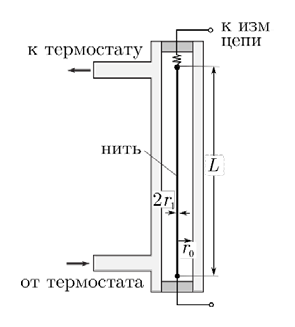
\includegraphics[width=0.4\textwidth]{Рисунок 1. Схема установки.png}
        Рис 1. Схема установки
    \end{wrapfigure}

    Схема установки представлена на рисунке 1. Она представляет из себя полую цилиндрическую трубку с внутренним диаметром $2R = (10,0 \pm 0,1)\text{ мм}$, на оси которой расположена молибденовая нить с диаметром $2r = (0,050 \pm 0,005)\text{ мм}$ и длиной $L = 347\text{ мм}$ (погрешность на установке не была указана). Полость трубки заполнена воздухом и через небольшое отверстие сообщается с атмосферой (таким способом осуществляется поддержание постоянства давления). Стенки трубки помещены в кожух, через который пропускается вода, что обеспечивает постоянство температуры стенок.
    
    Молибденовая нить является одновременно источником тепла и термометром сопротивления. Сопротивление нити является однозначной функцией температуры и может быть найдено из таблиц, так как материал нити и её геометрические размеры известны. Также сопротивление может быть получено из закона Ома:
    
    \begin{equation}
        R = \frac{U}{I}
    \end{equation}
    
    
    \begin{wrapfigure}{l}{0.4\textwidth}
        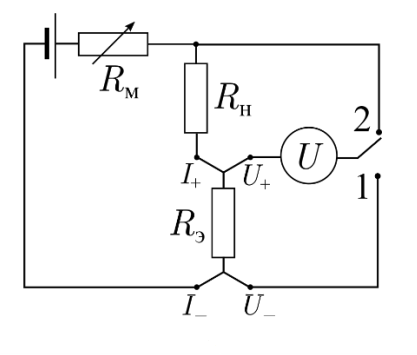
\includegraphics[width=0.4\textwidth]{Рисунок 2. Электрическая схема.png}
        Рис 2. Электрическая схема измерения сопротивления
    \end{wrapfigure}
    
    В данной работе для измерения сопротивления нити используется электрическая схема, изображённая на рисунке 2. В ней присутствуют единственный вольтметр и эталонное сопротивление $R_{\text{э}} = 10,000\text{ Ом}$. Если переключатель находится в положении 2, то вольтметр измеряет напряжение на нити $R_{\text{ н}}$, если в положении 1 - на эталонном сопротивлении. 
    
    Пусть напряжение, измеряемое вольтметром в положении 1 равно $U_1$, а в положении 2 - $U_2$, а токи, текущие по нити в каждом из этих положение равны $I_1$ и $I_2$ соответственно. Так как класс точности вольтметра равен 0,01, то его сопротивление можно считать бесконечно большим, а тогда $I_1 \approx I_2$. Отсюда, прменив закон Ома, получаем:
    
    \begin{equation}
        R_{\text{ н}} = R_{\text{ э}}\frac{U_2}{U_1}
    \end{equation}
    
\section{Методика измерений}	

    Чем выше сила тока, тем точнее будет измерена как она, так и напряжение на нагрузке. Однако мощность тока выделяемая на проводнике в ходе протекания тока $P\sim I^2$. Вследствие этого температура резистора становится выше, чем у объекта, температуру которого нужно измерить.
    
    Решением данной проблемы является построение зависимости $R(P)$ и её экстраполяция к мощности $P\rightarrow 0$. Это позволит найти сопротивление нити $R_0$, при котором её температура равна температуре термостата.

\section{Обработка полученных результатов}

    В ходе работы было проведено 5 серий по 8 (один раз 7) измерений. Температура термостата от серии к серии увеличивалась. Результаты измерений приведены в таблице 1. Также по данным этой таблицы построены графики 1-5, на которых по экспериментальным точкам проведены аппроксимирующие прямые согласно методу наименьших квадратов.
    
    Параметры аппроксимирующих прямых сведём в таблицу 2, а также построим график 6 зависимости $R$ от $T$, для значений $R$, соответствующий пересечению с осью $Oy$ на графиках 1-5. Аппроксимирующая прямая с графика 6 определяется параметрами:
    \[\frac{dR}{dT} = (44,76 \pm 0,05) \frac{\text{мОм}}{\text{К}}\]
    \[R(0) = (1360 \pm 20) \text{мОм}\]
    По этим данным можно получить, что сопротивление нити при $0 \degree C$ равно:
    \[R_{273} = (13,58 \pm 0,02) \text{Ом}\]
    Также получим температурный коэффициент сопротивления материала нити (молибден):
    \[\alpha = \frac{1}{R_{273}}\frac{dR}{dT} = (3,296 \pm 0,006)\cdot 10^{-3}\frac{1}{\text{К}}\]
    
    Далее найдём величины $\frac{dQ}{dT}$ для каждой из температур. Результаты расчётов приведены в таблице 3. Теперь по формуле \eqref{main} найдём теплопроводности воздуха при разных температурах. Результаты сведём в таблицу 4. По данным таблицы 4 построим график 7 зависимости $\kappa(T)$. На этом графике проведена аппроксимирующая прямая по методу наименьших квадратов. Параметры прямой с погрешностями:
    \[\frac{d\kappa}{dT} = (-0,5 \pm 1,6)\cdot 10^{-5}\ \frac{\text{Вт}}{\text{м}\cdot\text{К}^2}\]
    \[\kappa(0) = (0,035 \pm 0,005)\ \frac{\text{Вт}}{\text{м}\cdot\text{К}}\]

\section{Вывод}
    
    В ходе данной работы были измерены коэффициенты теплопроводности при различных температурах. Хотя по порядку величины полученные значения соответствуют табличным ($0,0259\ \frac{\text{Вт}}{\text{м}\cdot\text{К}}$ при $T = 20\degree C$ и $0,029\ \frac{\text{Вт}}{\text{м}\cdot\text{К}}$ при $T = 60\degree C$), даже с учётом погрешности они не совпадают. Также вследствие того, что погрешности коэффициентов теплопроводности по порядку величины такие же, как и разброс значения самих коэффициентов, не удалось получить адекватную зависимость $\kappa(T)$.

\newpage
\section{Приложения}

    \subsection{Таблица 1. Нагрузочная характеристика}
    \begin{center}
        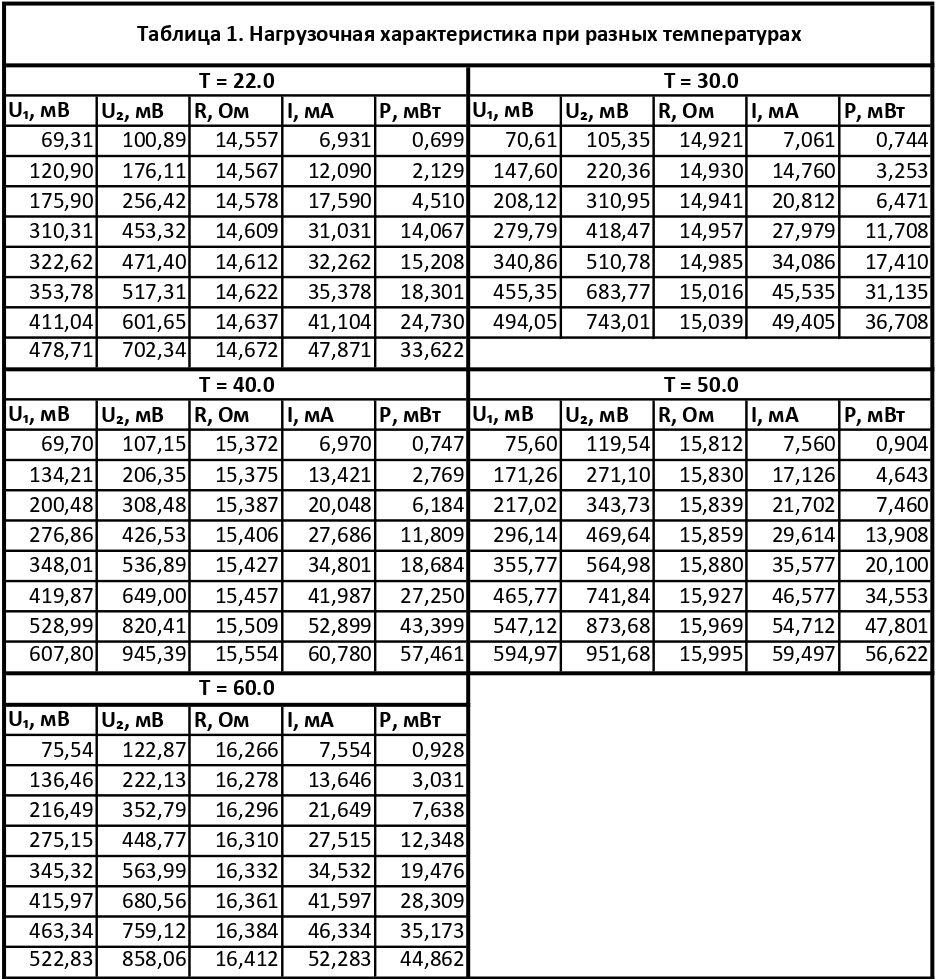
\includegraphics[width=8cm]{Таблица 1.jpg}
    \end{center}
    
    \subsection{Таблица 2. Параметры наилучших прямых.}
    \begin{center}
        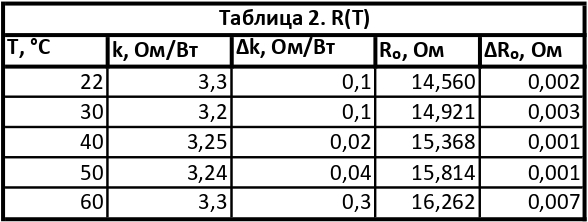
\includegraphics[width = 8cm]{Таблицы 2.jpg}
    \end{center}
    
    \subsection{Таблица 3. Параметры dQ/dT}
    \begin{center}
        \begin{tabular}{|c|c|c|}
            \hline
            T, К & $\beta\equiv$ dQ/dT, мВт/К & $\Delta_{\beta}$, мВт/К \\ \hline
            295 & 13,6  & 0,4  \\ \hline
            303 & 14,0  & 0,4  \\ \hline
            313 & 13,77 & 0,09 \\ \hline
            323 & 13,8  & 0,2  \\ \hline
            333 & 13,6  & 1,2  \\ \hline
        \end{tabular}
    \end{center}
    
    \subsection{Таблица 4. Теплопроводности при разных температурах}
    \begin{center}
        \begin{tabular}{|c|c|c|}
            \hline
            T, К & $\kappa$, Вт/м$\cdot$К & $\Delta_{\kappa}$, Вт/м$\cdot$К \\ \hline
            295 & 0,033  & 0,001 \\ \hline
            303 & 0,034  & 0,001 \\ \hline
            313 & 0,0335 & 0,0002 \\ \hline
            323 & 0,0336 & 0,0004 \\ \hline
            333 & 0,033  & 0,003 \\ \hline
        \end{tabular}
    \end{center}
    
    \newpage
    \subsection{График 1. R(P) при T = 22 \degree C}
    \begin{center}
        \centering
        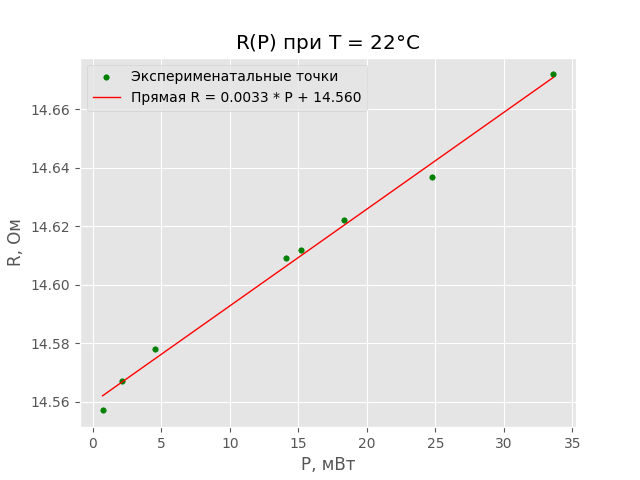
\includegraphics[width = 9cm]{22.png}
    \end{center}
    
    \subsection{График 2. R(P) при T = 30 \degree C}
    \begin{center}
        \centering
        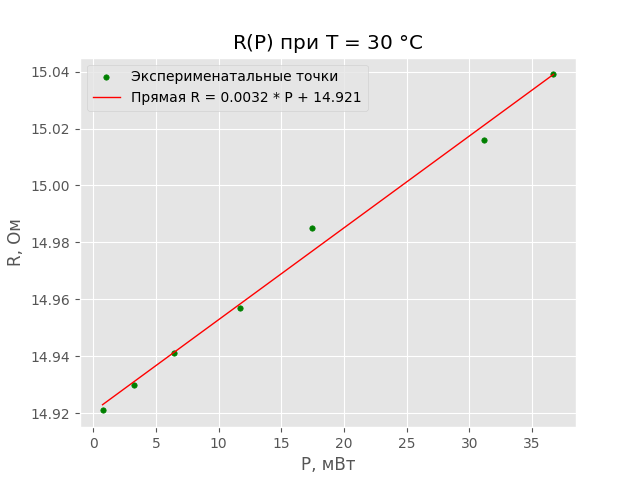
\includegraphics[width = 9cm]{30.png}
    \end{center}
    
    \newpage
    \subsection{График 3. R(P) при T = 40\degree C}
    \begin{center}
        \centering
        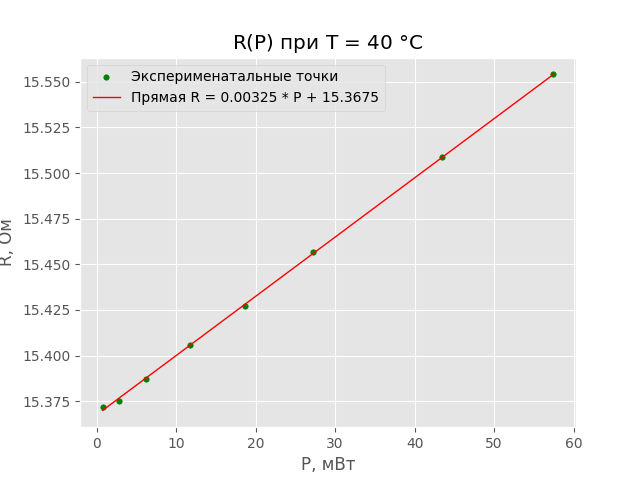
\includegraphics[width = 9cm]{40.png}
    \end{center}
    
    \subsection{График 4. R(P) при T = 50 \degree C}
    \begin{center}
        \centering
        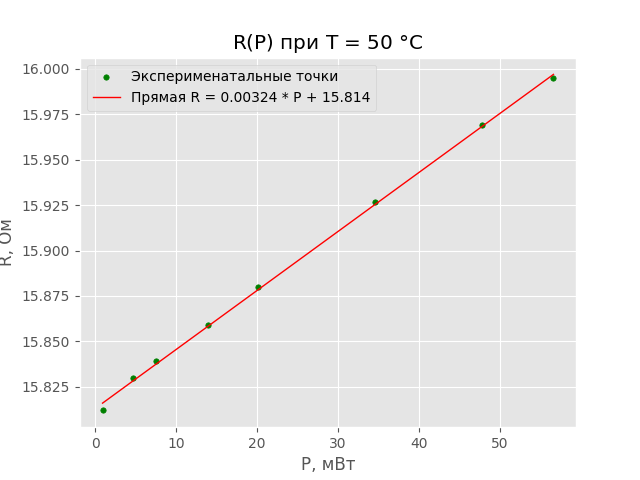
\includegraphics[width = 9cm]{50.png}
    \end{center}
    
    \newpage
    \subsection{График 5. R(P) при T = 60 \degree C}
    \begin{center}
        \centering
        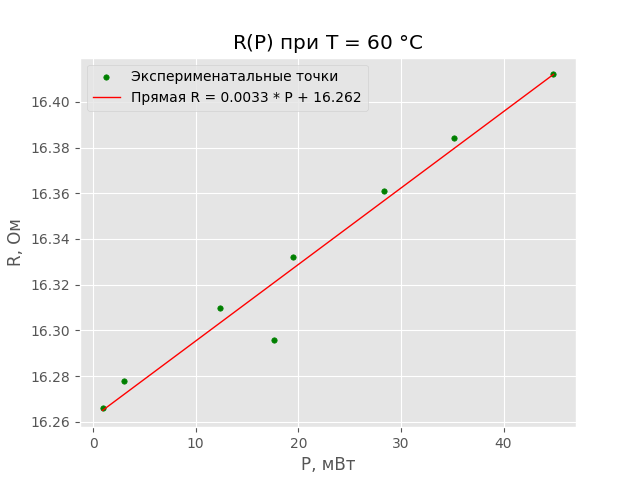
\includegraphics[width = 9cm]{60.png}
    \end{center}
    
    \subsection{График 6. R(T)}
    \begin{center}
        \centering
        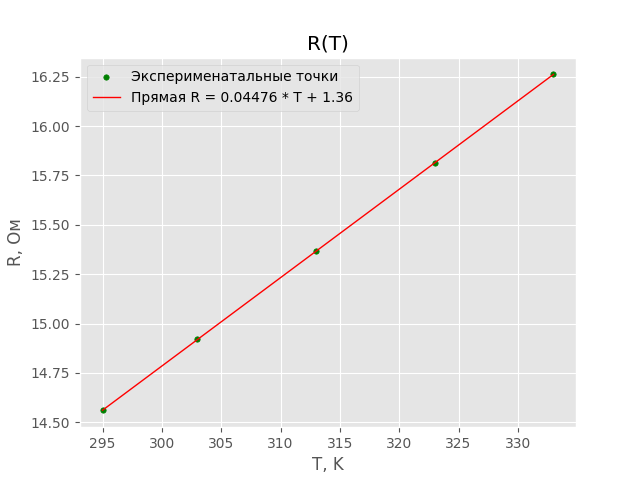
\includegraphics[width = 9cm]{График 6.png}
    \end{center}
    
    \subsection{График 6. R(T)}
    \begin{center}
        \centering
        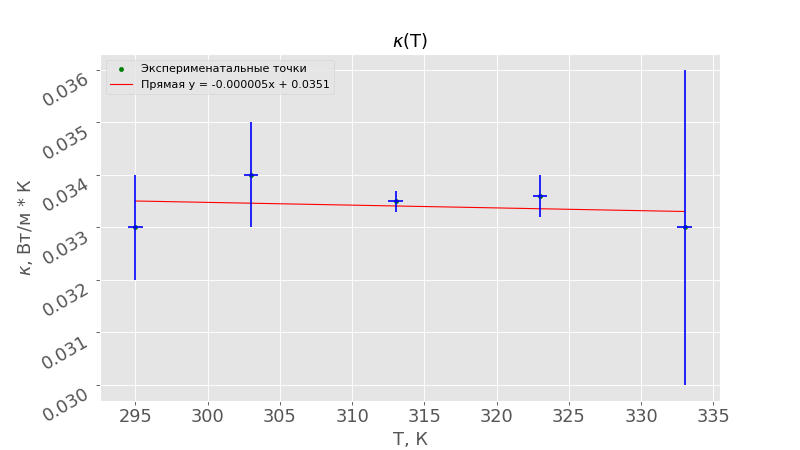
\includegraphics[width = 10cm]{График 7.png}
    \end{center}

\end{document}